% GLOBECOM 2027 draft (double-blind). Numbers come from generated_numbers.tex / generated_tables.tex, which
% experiments/paper_figures.py writes from the result files; do not type numbers by hand.
\documentclass[conference]{IEEEtran}
\usepackage{amsmath,amssymb,amsthm}
\usepackage{graphicx}
\usepackage{booktabs}
\usepackage{xcolor}
\usepackage{cite}
\usepackage{url}
\newtheorem{lemma}{Lemma}
\newtheorem{proposition}{Proposition}
\providecommand{\TBD}[1]{\textbf{\color{red}[#1]}}
\IfFileExists{generated_numbers.tex}{% generated by experiments/paper_figures.py -- do not edit
\providecommand{\TBD}[1]{\textbf{\color{red}[#1]}}
\newcommand{\CleanPsnr}{30.88}
\newcommand{\DesignFortyAtFifty}{+1.88}
\newcommand{\DesignFortyAtZeroLoss}{2.59}
\newcommand{\GradFecFifty}{24.66}
\newcommand{\GradFecForty}{25.25}
\newcommand{\GradFecFortyFive}{25.04}
\newcommand{\GradFecGainFifty}{+6.35}
\newcommand{\GradFecGainForty}{+4.52}
\newcommand{\GradFecGainFortyFive}{+5.97}
\newcommand{\GradFecGainTen}{$-$4.33}
\newcommand{\GradFecGainThirty}{$-$3.03}
\newcommand{\GradFecGainThirtyFive}{+1.04}
\newcommand{\GradFecGainTwenty}{$-$4.80}
\newcommand{\GradFecGainZero}{$-$3.80}
\newcommand{\GradFecTen}{26.55}
\newcommand{\GradFecThirty}{25.64}
\newcommand{\GradFecThirtyFive}{25.44}
\newcommand{\GradFecTwenty}{26.07}
\newcommand{\GradFecZero}{27.08}
\newcommand{\HandGainMaxAll}{+4.0}
\newcommand{\HandGainMinAll}{+2.3}
\newcommand{\HandTierAttentionFifty}{18.86}
\newcommand{\HandTierAttentionForty}{21.47}
\newcommand{\HandTierAttentionFortyFive}{19.95}
\newcommand{\HandTierAttentionGainFifty}{+0.55}
\newcommand{\HandTierAttentionGainForty}{+0.74}
\newcommand{\HandTierAttentionGainFortyFive}{+0.88}
\newcommand{\HandTierAttentionGainTen}{$-$1.47}
\newcommand{\HandTierAttentionGainThirty}{$-$3.10}
\newcommand{\HandTierAttentionGainThirtyFive}{$-$0.93}
\newcommand{\HandTierAttentionGainTwenty}{$-$2.77}
\newcommand{\HandTierAttentionGainZero}{+0.00}
\newcommand{\HandTierAttentionTen}{29.41}
\newcommand{\HandTierAttentionThirty}{25.57}
\newcommand{\HandTierAttentionThirtyFive}{23.47}
\newcommand{\HandTierAttentionTwenty}{28.10}
\newcommand{\HandTierAttentionZero}{30.88}
\newcommand{\HandTierFifty}{20.21}
\newcommand{\HandTierForty}{23.59}
\newcommand{\HandTierFortyFive}{21.77}
\newcommand{\HandTierGainFifty}{+1.89}
\newcommand{\HandTierGainForty}{+2.86}
\newcommand{\HandTierGainFortyFive}{+2.69}
\newcommand{\HandTierGainTen}{$-$0.61}
\newcommand{\HandTierGainThirty}{$-$0.95}
\newcommand{\HandTierGainThirtyFive}{+1.31}
\newcommand{\HandTierGainTwenty}{$-$1.19}
\newcommand{\HandTierGainZero}{+0.00}
\newcommand{\HandTierPerImageFifty}{20.36}
\newcommand{\HandTierPerImageForty}{23.81}
\newcommand{\HandTierPerImageFortyFive}{21.97}
\newcommand{\HandTierPerImageGainFifty}{+2.05}
\newcommand{\HandTierPerImageGainForty}{+3.08}
\newcommand{\HandTierPerImageGainFortyFive}{+2.90}
\newcommand{\HandTierPerImageGainTen}{$-$0.53}
\newcommand{\HandTierPerImageGainThirty}{$-$0.77}
\newcommand{\HandTierPerImageGainThirtyFive}{+1.52}
\newcommand{\HandTierPerImageGainTwenty}{$-$1.06}
\newcommand{\HandTierPerImageGainZero}{+0.00}
\newcommand{\HandTierPerImageTen}{30.35}
\newcommand{\HandTierPerImageThirty}{27.90}
\newcommand{\HandTierPerImageThirtyFive}{25.92}
\newcommand{\HandTierPerImageTwenty}{29.81}
\newcommand{\HandTierPerImageZero}{30.88}
\newcommand{\HandTierRandomFifty}{19.12}
\newcommand{\HandTierRandomForty}{21.67}
\newcommand{\HandTierRandomFortyFive}{20.24}
\newcommand{\HandTierRandomGainFifty}{+0.81}
\newcommand{\HandTierRandomGainForty}{+0.94}
\newcommand{\HandTierRandomGainFortyFive}{+1.17}
\newcommand{\HandTierRandomGainTen}{$-$1.74}
\newcommand{\HandTierRandomGainThirty}{$-$3.33}
\newcommand{\HandTierRandomGainThirtyFive}{$-$0.93}
\newcommand{\HandTierRandomGainTwenty}{$-$3.15}
\newcommand{\HandTierRandomGainZero}{+0.00}
\newcommand{\HandTierRandomTen}{29.14}
\newcommand{\HandTierRandomThirty}{25.34}
\newcommand{\HandTierRandomThirtyFive}{23.47}
\newcommand{\HandTierRandomTwenty}{27.72}
\newcommand{\HandTierRandomZero}{30.88}
\newcommand{\HandTierTen}{30.28}
\newcommand{\HandTierThirty}{27.72}
\newcommand{\HandTierThirtyFive}{25.72}
\newcommand{\HandTierTwenty}{29.69}
\newcommand{\HandTierZero}{30.88}
\newcommand{\JpegAdaptiveFifty}{30.39}
\newcommand{\JpegAdaptiveForty}{32.98}
\newcommand{\JpegAdaptiveFortyFive}{31.10}
\newcommand{\JpegAdaptiveTen}{36.76}
\newcommand{\JpegAdaptiveThirty}{35.08}
\newcommand{\JpegAdaptiveThirtyFive}{33.52}
\newcommand{\JpegAdaptiveTwenty}{36.74}
\newcommand{\JpegAdaptiveZero}{36.76}
\newcommand{\JpegFixedFifty}{11.75}
\newcommand{\JpegFixedForty}{14.06}
\newcommand{\JpegFixedFortyFive}{11.83}
\newcommand{\JpegFixedTen}{36.76}
\newcommand{\JpegFixedThirty}{31.48}
\newcommand{\JpegFixedThirtyFive}{21.64}
\newcommand{\JpegFixedTwenty}{36.74}
\newcommand{\JpegFixedZero}{36.76}
\newcommand{\JtwokAdaptiveFifty}{26.01}
\newcommand{\JtwokAdaptiveForty}{28.55}
\newcommand{\JtwokAdaptiveFortyFive}{26.57}
\newcommand{\JtwokAdaptiveTen}{32.91}
\newcommand{\JtwokAdaptiveThirty}{30.96}
\newcommand{\JtwokAdaptiveThirtyFive}{29.72}
\newcommand{\JtwokAdaptiveTwenty}{32.89}
\newcommand{\JtwokAdaptiveZero}{32.91}
\newcommand{\JtwokFixedFifty}{12.33}
\newcommand{\JtwokFixedForty}{14.36}
\newcommand{\JtwokFixedFortyFive}{12.47}
\newcommand{\JtwokFixedTen}{32.91}
\newcommand{\JtwokFixedThirty}{28.60}
\newcommand{\JtwokFixedThirtyFive}{20.57}
\newcommand{\JtwokFixedTwenty}{32.89}
\newcommand{\JtwokFixedZero}{32.91}
\newcommand{\KnSixteenClean}{28.28}
\newcommand{\KnSixteenFifty}{28.28}
\newcommand{\KnSixteenForty}{28.28}
\newcommand{\KnSixteenFortyFive}{28.28}
\newcommand{\KnSixteenTen}{28.28}
\newcommand{\KnSixteenThirty}{28.28}
\newcommand{\KnSixteenThirtyFive}{28.28}
\newcommand{\KnSixteenTwenty}{28.28}
\newcommand{\KnSixteenZero}{28.28}
\newcommand{\KnTwelveClean}{30.06}
\newcommand{\KnTwelveFifty}{30.06}
\newcommand{\KnTwelveForty}{30.06}
\newcommand{\KnTwelveFortyFive}{30.06}
\newcommand{\KnTwelveTen}{30.06}
\newcommand{\KnTwelveThirty}{30.06}
\newcommand{\KnTwelveThirtyFive}{30.06}
\newcommand{\KnTwelveTwenty}{30.06}
\newcommand{\KnTwelveZero}{30.06}
\newcommand{\ModelsAll}{8}
\newcommand{\MultiTierMaxGain}{0.15}
\newcommand{\NoRSFifty}{18.31}
\newcommand{\NoRSForty}{19.62}
\newcommand{\NoRSFortyFive}{18.94}
\newcommand{\NoRSGainFifty}{$-$0.01}
\newcommand{\NoRSGainForty}{$-$1.10}
\newcommand{\NoRSGainFortyFive}{$-$0.13}
\newcommand{\NoRSGainTen}{$-$5.08}
\newcommand{\NoRSGainThirty}{$-$7.51}
\newcommand{\NoRSGainThirtyFive}{$-$4.04}
\newcommand{\NoRSGainTwenty}{$-$7.79}
\newcommand{\NoRSGainZero}{+0.00}
\newcommand{\NoRSTen}{25.80}
\newcommand{\NoRSThirty}{21.16}
\newcommand{\NoRSThirtyFive}{20.36}
\newcommand{\NoRSTwenty}{23.09}
\newcommand{\NoRSZero}{30.88}
\newcommand{\NoRsBestValClean}{27.83}
\newcommand{\OptGroupedFifty}{24.66}
\newcommand{\OptGroupedForty}{27.25}
\newcommand{\OptGroupedFortyFive}{25.75}
\newcommand{\OptGroupedGainFifty}{+6.35}
\newcommand{\OptGroupedGainForty}{+6.52}
\newcommand{\OptGroupedGainFortyFive}{+6.68}
\newcommand{\OptGroupedGainTen}{+0.00}
\newcommand{\OptGroupedGainThirty}{+0.80}
\newcommand{\OptGroupedGainThirtyFive}{+4.14}
\newcommand{\OptGroupedGainTwenty}{$-$0.00}
\newcommand{\OptGroupedGainZero}{+0.00}
\newcommand{\OptGroupedTen}{30.88}
\newcommand{\OptGroupedThirty}{29.47}
\newcommand{\OptGroupedThirtyFive}{28.54}
\newcommand{\OptGroupedTwenty}{30.88}
\newcommand{\OptGroupedZero}{30.88}
\newcommand{\OptPetFifty}{24.61}
\newcommand{\OptPetForty}{27.03}
\newcommand{\OptPetFortyFive}{25.86}
\newcommand{\OptPetGainFifty}{+6.29}
\newcommand{\OptPetGainForty}{+6.30}
\newcommand{\OptPetGainFortyFive}{+6.79}
\newcommand{\OptPetGainTen}{+0.00}
\newcommand{\OptPetGainThirty}{+0.73}
\newcommand{\OptPetGainThirtyFive}{+4.01}
\newcommand{\OptPetGainTwenty}{$-$0.00}
\newcommand{\OptPetGainZero}{+0.00}
\newcommand{\OptPetTen}{30.88}
\newcommand{\OptPetThirty}{29.40}
\newcommand{\OptPetThirtyFive}{28.42}
\newcommand{\OptPetTwenty}{30.87}
\newcommand{\OptPetZero}{30.88}
\newcommand{\PetTwinFifty}{20.68}
\newcommand{\PetTwinForty}{23.51}
\newcommand{\PetTwinFortyFive}{22.00}
\newcommand{\PetTwinGainFifty}{+2.37}
\newcommand{\PetTwinGainForty}{+2.78}
\newcommand{\PetTwinGainFortyFive}{+2.93}
\newcommand{\PetTwinGainTen}{$-$0.67}
\newcommand{\PetTwinGainThirty}{$-$0.41}
\newcommand{\PetTwinGainThirtyFive}{+1.53}
\newcommand{\PetTwinGainTwenty}{$-$1.25}
\newcommand{\PetTwinGainZero}{+0.00}
\newcommand{\PetTwinTen}{30.21}
\newcommand{\PetTwinThirty}{28.26}
\newcommand{\PetTwinThirtyFive}{25.93}
\newcommand{\PetTwinTwenty}{29.63}
\newcommand{\PetTwinZero}{30.88}
\newcommand{\PetVsTruncMax}{0.25}
\newcommand{\ReferenceCells}{56}
\newcommand{\ReferenceMaxDiff}{0.000}
\newcommand{\RobustGroupedFifty}{23.90}
\newcommand{\RobustGroupedForty}{26.16}
\newcommand{\RobustGroupedFortyFive}{25.49}
\newcommand{\RobustGroupedGainFifty}{+5.58}
\newcommand{\RobustGroupedGainForty}{+5.43}
\newcommand{\RobustGroupedGainFortyFive}{+6.41}
\newcommand{\RobustGroupedGainTen}{$-$2.47}
\newcommand{\RobustGroupedGainThirty}{$-$1.79}
\newcommand{\RobustGroupedGainThirtyFive}{+2.13}
\newcommand{\RobustGroupedGainTwenty}{$-$3.25}
\newcommand{\RobustGroupedGainZero}{$-$1.59}
\newcommand{\RobustGroupedTen}{28.42}
\newcommand{\RobustGroupedThirty}{26.88}
\newcommand{\RobustGroupedThirtyFive}{26.53}
\newcommand{\RobustGroupedTwenty}{27.62}
\newcommand{\RobustGroupedZero}{29.29}
\newcommand{\RobustPetFifty}{24.03}
\newcommand{\RobustPetForty}{26.24}
\newcommand{\RobustPetFortyFive}{25.60}
\newcommand{\RobustPetGainFifty}{+5.72}
\newcommand{\RobustPetGainForty}{+5.52}
\newcommand{\RobustPetGainFortyFive}{+6.53}
\newcommand{\RobustPetGainTen}{$-$2.49}
\newcommand{\RobustPetGainThirty}{$-$1.78}
\newcommand{\RobustPetGainThirtyFive}{+2.18}
\newcommand{\RobustPetGainTwenty}{$-$3.29}
\newcommand{\RobustPetGainZero}{$-$1.53}
\newcommand{\RobustPetTen}{28.39}
\newcommand{\RobustPetThirty}{26.90}
\newcommand{\RobustPetThirtyFive}{26.58}
\newcommand{\RobustPetTwenty}{27.59}
\newcommand{\RobustPetZero}{29.35}
\newcommand{\SeedsAdj}{5}
\newcommand{\SeedsDeep}{3}
\newcommand{\SelectorFifty}{24.66}
\newcommand{\SelectorForty}{27.25}
\newcommand{\SelectorFortyFive}{25.86}
\newcommand{\SelectorGainFifty}{+6.35}
\newcommand{\SelectorGainForty}{+6.52}
\newcommand{\SelectorGainFortyFive}{+6.79}
\newcommand{\SelectorGainTen}{+0.00}
\newcommand{\SelectorGainThirty}{+0.80}
\newcommand{\SelectorGainThirtyFive}{+4.14}
\newcommand{\SelectorGainTwenty}{$-$0.00}
\newcommand{\SelectorGainZero}{+0.00}
\newcommand{\SelectorTen}{30.88}
\newcommand{\SelectorThirty}{29.47}
\newcommand{\SelectorThirtyFive}{28.54}
\newcommand{\SelectorTwenty}{30.87}
\newcommand{\SelectorZero}{30.88}
\newcommand{\SurrogateCells}{77}
\newcommand{\SurrogateMedianRelErr}{5.4}
\newcommand{\SurrogateSpearman}{0.997}
\newcommand{\TopFourShareMaxAdj}{84}
\newcommand{\TopFourShareMaxDeep}{72}
\newcommand{\TopFourShareMinAdj}{66}
\newcommand{\TopFourShareMinDeep}{69}
\newcommand{\TruncAttentionFifty}{18.12}
\newcommand{\TruncAttentionForty}{25.52}
\newcommand{\TruncAttentionFortyFive}{20.99}
\newcommand{\TruncAttentionGainFifty}{$-$0.19}
\newcommand{\TruncAttentionGainForty}{+4.80}
\newcommand{\TruncAttentionGainFortyFive}{+1.92}
\newcommand{\TruncAttentionGainTen}{+0.00}
\newcommand{\TruncAttentionGainThirty}{+0.80}
\newcommand{\TruncAttentionGainThirtyFive}{+4.12}
\newcommand{\TruncAttentionGainTwenty}{$-$0.00}
\newcommand{\TruncAttentionGainZero}{+0.00}
\newcommand{\TruncAttentionTen}{30.88}
\newcommand{\TruncAttentionThirty}{29.47}
\newcommand{\TruncAttentionThirtyFive}{28.52}
\newcommand{\TruncAttentionTwenty}{30.88}
\newcommand{\TruncAttentionZero}{30.88}
\newcommand{\TruncEnergyFifty}{24.21}
\newcommand{\TruncEnergyForty}{26.72}
\newcommand{\TruncEnergyFortyFive}{25.34}
\newcommand{\TruncEnergyGainFifty}{+5.90}
\newcommand{\TruncEnergyGainForty}{+6.00}
\newcommand{\TruncEnergyGainFortyFive}{+6.27}
\newcommand{\TruncEnergyGainTen}{+0.00}
\newcommand{\TruncEnergyGainThirty}{+0.90}
\newcommand{\TruncEnergyGainThirtyFive}{+3.74}
\newcommand{\TruncEnergyGainTwenty}{$-$0.00}
\newcommand{\TruncEnergyGainZero}{+0.00}
\newcommand{\TruncEnergyTen}{30.88}
\newcommand{\TruncEnergyThirty}{29.57}
\newcommand{\TruncEnergyThirtyFive}{28.14}
\newcommand{\TruncEnergyTwenty}{30.88}
\newcommand{\TruncEnergyZero}{30.88}
\newcommand{\TruncGainMaxAdj}{+6.52}
\newcommand{\TruncGainMaxAll}{+9.4}
\newcommand{\TruncGainMaxDeep}{+9.45}
\newcommand{\TruncGainMinAdj}{+4.02}
\newcommand{\TruncGainMinAll}{+4.0}
\newcommand{\TruncGainMinDeep}{+6.10}
\newcommand{\TruncHeadFifty}{24.72}
\newcommand{\TruncHeadForty}{27.10}
\newcommand{\TruncHeadFortyFive}{25.64}
\newcommand{\TruncHeadGainFifty}{+6.40}
\newcommand{\TruncHeadGainForty}{+6.37}
\newcommand{\TruncHeadGainFortyFive}{+6.57}
\newcommand{\TruncHeadGainTen}{+0.00}
\newcommand{\TruncHeadGainThirty}{+0.92}
\newcommand{\TruncHeadGainThirtyFive}{+3.92}
\newcommand{\TruncHeadGainTwenty}{$-$0.00}
\newcommand{\TruncHeadGainZero}{+0.00}
\newcommand{\TruncHeadTen}{30.88}
\newcommand{\TruncHeadThirty}{29.59}
\newcommand{\TruncHeadThirtyFive}{28.32}
\newcommand{\TruncHeadTwenty}{30.88}
\newcommand{\TruncHeadZero}{30.88}
\newcommand{\TruncKeepFifty}{10}
\newcommand{\TruncKeepForty}{13}
\newcommand{\TruncKeepFortyFive}{12}
\newcommand{\TruncKeepTen}{16}
\newcommand{\TruncKeepThirty}{15}
\newcommand{\TruncKeepThirtyFive}{14}
\newcommand{\TruncKeepTwenty}{16}
\newcommand{\TruncOracleFifty}{24.52}
\newcommand{\TruncOracleForty}{27.25}
\newcommand{\TruncOracleFortyFive}{25.75}
\newcommand{\TruncOracleGainFifty}{+6.21}
\newcommand{\TruncOracleGainForty}{+6.52}
\newcommand{\TruncOracleGainFortyFive}{+6.68}
\newcommand{\TruncOracleGainTen}{+0.00}
\newcommand{\TruncOracleGainThirty}{+0.80}
\newcommand{\TruncOracleGainThirtyFive}{+4.12}
\newcommand{\TruncOracleGainTwenty}{$-$0.00}
\newcommand{\TruncOracleGainZero}{+0.00}
\newcommand{\TruncOracleTen}{30.88}
\newcommand{\TruncOracleThirty}{29.47}
\newcommand{\TruncOracleThirtyFive}{28.52}
\newcommand{\TruncOracleTwenty}{30.88}
\newcommand{\TruncOracleZero}{30.88}
\newcommand{\TruncOverHandForty}{3.66}
\newcommand{\TruncOverHandMaxAll}{+5.8}
\newcommand{\TruncOverHandMinAll}{+1.7}
\newcommand{\TruncRandomFifty}{19.37}
\newcommand{\TruncRandomForty}{22.31}
\newcommand{\TruncRandomFortyFive}{20.84}
\newcommand{\TruncRandomGainFifty}{+1.05}
\newcommand{\TruncRandomGainForty}{+1.58}
\newcommand{\TruncRandomGainFortyFive}{+1.77}
\newcommand{\TruncRandomGainTen}{+0.00}
\newcommand{\TruncRandomGainThirty}{$-$2.02}
\newcommand{\TruncRandomGainThirtyFive}{$-$0.26}
\newcommand{\TruncRandomGainTwenty}{$-$0.00}
\newcommand{\TruncRandomGainZero}{+0.00}
\newcommand{\TruncRandomTen}{30.88}
\newcommand{\TruncRandomThirty}{26.65}
\newcommand{\TruncRandomThirtyFive}{24.14}
\newcommand{\TruncRandomTwenty}{30.88}
\newcommand{\TruncRandomZero}{30.88}
\newcommand{\TwoTierUnsortedFifty}{18.35}
\newcommand{\TwoTierUnsortedForty}{20.68}
\newcommand{\TwoTierUnsortedFortyFive}{19.20}
\newcommand{\TwoTierUnsortedGainFifty}{+0.04}
\newcommand{\TwoTierUnsortedGainForty}{$-$0.05}
\newcommand{\TwoTierUnsortedGainFortyFive}{+0.13}
\newcommand{\TwoTierUnsortedGainTen}{+0.00}
\newcommand{\TwoTierUnsortedGainThirty}{$-$1.69}
\newcommand{\TwoTierUnsortedGainThirtyFive}{$-$1.00}
\newcommand{\TwoTierUnsortedGainTwenty}{$-$0.14}
\newcommand{\TwoTierUnsortedGainZero}{+0.00}
\newcommand{\TwoTierUnsortedTen}{30.88}
\newcommand{\TwoTierUnsortedThirty}{26.99}
\newcommand{\TwoTierUnsortedThirtyFive}{23.40}
\newcommand{\TwoTierUnsortedTwenty}{30.73}
\newcommand{\TwoTierUnsortedZero}{30.88}
\newcommand{\UniformDiagFifty}{19.56}
\newcommand{\UniformDiagForty}{21.90}
\newcommand{\UniformDiagFortyFive}{20.35}
\newcommand{\UniformDiagGainFifty}{+1.25}
\newcommand{\UniformDiagGainForty}{+1.18}
\newcommand{\UniformDiagGainFortyFive}{+1.28}
\newcommand{\UniformDiagGainTen}{+0.00}
\newcommand{\UniformDiagGainThirty}{+0.28}
\newcommand{\UniformDiagGainThirtyFive}{+0.78}
\newcommand{\UniformDiagGainTwenty}{+0.00}
\newcommand{\UniformDiagGainZero}{+0.00}
\newcommand{\UniformDiagTen}{30.88}
\newcommand{\UniformDiagThirty}{28.95}
\newcommand{\UniformDiagThirtyFive}{25.19}
\newcommand{\UniformDiagTwenty}{30.88}
\newcommand{\UniformDiagZero}{30.88}
\newcommand{\UniformFifty}{18.31}
\newcommand{\UniformForty}{20.73}
\newcommand{\UniformFortyFive}{19.07}
\newcommand{\UniformTen}{30.88}
\newcommand{\UniformThirty}{28.67}
\newcommand{\UniformThirtyFive}{24.40}
\newcommand{\UniformTwenty}{30.88}
\newcommand{\UniformZero}{30.88}
\newcommand{\WebpAdaptiveFifty}{35.35}
\newcommand{\WebpAdaptiveForty}{36.84}
\newcommand{\WebpAdaptiveFortyFive}{36.23}
\newcommand{\WebpAdaptiveTen}{38.14}
\newcommand{\WebpAdaptiveThirty}{37.73}
\newcommand{\WebpAdaptiveThirtyFive}{37.28}
\newcommand{\WebpAdaptiveTwenty}{38.12}
\newcommand{\WebpAdaptiveZero}{38.14}
\newcommand{\WebpFixedFifty}{12.52}
\newcommand{\WebpFixedForty}{15.32}
\newcommand{\WebpFixedFortyFive}{12.83}
\newcommand{\WebpFixedTen}{38.14}
\newcommand{\WebpFixedThirty}{32.88}
\newcommand{\WebpFixedThirtyFive}{23.04}
\newcommand{\WebpFixedTwenty}{38.12}
\newcommand{\WebpFixedZero}{38.14}
}{}

\begin{document}

\title{Which Latent Bytes Deserve Parity?\\Erasure Sensitivity and Packet-Level FEC\\for Quantized Deep JSCC}
\author{\IEEEauthorblockN{Anonymous Authors}\IEEEauthorblockA{Submitted for double-blind review}}
\maketitle

\begin{abstract}
Deploying deep joint source-channel coding (JSCC) over packet networks requires quantized latents and
packet-level forward error correction, which raises a practical question: which latent bytes deserve the
parity? We study byte-quantized JSCC image models whose latent symbols are protected by systematic
Reed--Solomon (RS) codes over a packet-erasure channel. First, leave-one-out (LOO) erasure sensitivity is
strongly concentrated: the four most damaging of 16 latent channels carry
\TopFourShareMinAdj--\TopFourShareMaxAdj\% of the LOO MSE damage with attention modules and
\TopFourShareMinDeep--\TopFourShareMaxDeep\% without them, the sorted profile is stable across training
seeds while channel indices permute, and it transfers across datasets. The SNR-conditioned attention
gates of the backbone do not rank this sensitivity, whereas latent energy and a 2,048-MAC predictor do.
Second, because RS codes are MDS, the receiver outcome of any systematic layout is a deterministic
function of the loss pattern; this yields an exact fast simulator and a closed-form additive surrogate of
the expected distortion that predicts simulated MSE with Spearman correlation \SurrogateSpearman. Third,
optimizing the allocation shows that, at a known loss rate, the best use of a 50\% parity budget is not
multi-level unequal protection but \emph{importance-ordered truncation}: drop the least sensitive
channels and protect the rest with one strong code. At 40\% loss, across \ModelsAll{} converged models of
both architectures, this gains \TruncGainMinAll{} to \TruncGainMaxAll~dB over uniform RS, against
\HandGainMinAll{} to \HandGainMaxAll~dB for a hand-designed three-tier scheme, while the same truncation
guided by a random order gains only \TruncRandomGainForty~dB on the primary model. We also report the limits:
under a fair rate-adaptive comparison, a conventional codec with RS remains ahead of this JSCC model.
\end{abstract}

\begin{IEEEkeywords}
Deep joint source-channel coding, unequal error protection, Reed--Solomon codes, packet erasure channel,
semantic communication.
\end{IEEEkeywords}

% =====================================================================================================
\section{Introduction}
Deep JSCC maps a source directly to channel symbols and degrades gracefully with channel quality
\cite{bourtsoulatze2019deep}. Practical deployments, however, must pass through digital, packetized
links. Digital variants therefore quantize the latent \cite{tung2022deepjsccq,esfahanizadeh2026block} and,
over packet networks, rely on packet-level forward error correction (FEC). Once a latent travels as
bytes in packets, a classical question returns: with a fixed number of packets, which bytes should
the parity protect? For layered codecs this is the unequal loss protection (ULP) problem, solved
decades ago \cite{albanese1996pet,mohr2000ulp,dumitrescu2004optimal,hamzaoui2005optimized}. Those
solutions rely on an \emph{embedded} bitstream whose importance order is known. A JSCC latent has no
such order. Its importance must be measured or predicted, and the recent literature often takes it from
attention weights \cite{bajic2021collaborative,uyanik2023gradfec,zhan2026isfr}.

This paper answers three questions for byte-quantized JSCC image models with systematic RS codes over
packet erasures. (i) \emph{Is erasure sensitivity unequal across latent channels, and how can a
transmitter know it?} (ii) \emph{How should a fixed parity budget be allocated?} (iii) \emph{How do the
resulting systems compare with honest baselines?} Our contributions are:
\begin{itemize}
\item \textbf{Measurement.} LOO erasure damage is concentrated and its sorted profile is reproducible
across seeds and architectures. It exists without attention modules, so it is not an artefact of the
gates. Channel indices permute across seeds, so a ranking belongs to a checkpoint, and it transfers from
CIFAR-10 to CIFAR-100.
\item \textbf{Prediction.} The SNR-recalibration gates of ADJSCC \cite{xu2022adjscc}, repurposed as
importance, have essentially zero within-image rank correlation with the damage. Latent energy
($\rho_s=0.84$) and a 2,048-MAC head (top-4 overlap 0.92) predict it at negligible cost.
\item \textbf{Exact analysis and optimal allocation.} For any systematic MDS layout (grouped tiers,
PET~\cite{albanese1996pet}, or partial transmission) the decoded erasure pattern follows from the loss
pattern alone. We derive the per-symbol loss probability, an additive surrogate of the expected MSE that
dynamic programming optimizes exactly, and a validation-time search with an exact simulator.
\item \textbf{What the optimum looks like.} At a known loss rate, the optimum is importance-ordered
truncation with one strong code; multi-tier unequal protection and PET add little. The ranking decides
the outcome. Multi-level designs matter only when one allocation must serve a range of loss rates.
\item \textbf{Honest baselines.} We control for block length, random tiering, the PET layout,
Grad-FEC-style drop-and-protect \cite{uyanik2023gradfec}, a JSCC model that spends the whole budget on
latent bytes without RS, and rate-adaptive JPEG/JPEG2000/WebP with RS.
\end{itemize}

% =====================================================================================================
\section{Related Work}
\emph{Importance-aware protection of learned latents.} Grad-FEC \cite{uyanik2023gradfec} ranks deep-feature
packets with a Grad-CAM proxy and spends the slots of dropped low-importance packets on RS parity for
split inference. ISFR \cite{zhan2026isfr} uses the LOO-PSNR drop as feature importance and imposes an
order with nested dropout, protecting with modulation and power. Kim et al. \cite{kim2025uep} learn
per-bit protection targets for 8-bit JSCC features and find that short-block partitioning pays off only
beyond a threshold. We use the same LOO ground truth, but study packet-level systematic RS on
reconstruction JSCC, test whether attention predicts the damage, and characterize the optimal allocation
exactly.

\emph{JSCC over packet erasures.} Erasure-aware training \cite{esfahanizadeh2026block}, learnable mask tokens
with codec+FEC envelopes \cite{bo2026lgsemcom}, and information dispersal for learned codecs
\cite{wei2026everypacket} make latents robust without FEC or with ideal FEC. Yang et al.
\cite{yang2025partitioning} report that CNN JSCC concentrates information unevenly across channels, which
is the property we measure and exploit.

\emph{Classical ULP.} PET \cite{albanese1996pet} codes every priority class across all packets; ULP
\cite{mohr2000ulp} and globally optimal packetization \cite{dumitrescu2004optimal} allocate parity to an
embedded stream. Our grouped tiers are partitioned (each tier owns its packets), and we compare them with
their PET twins. Finite-blocklength effects \cite{polyanskiy2010finite} explain part of the difference.

\emph{Attention and importance.} Attention weights often fail to predict ablation damage
\cite{jain2019attention,morcos2018single}, and squeeze-and-excitation gates saturate in late layers
\cite{hu2018se}. The proxy-versus-LOO protocol follows pruning practice \cite{molchanov2017pruning}.
Imposed orderings (nested dropout \cite{rippel2014nested}, successive refinement \cite{kurka2021bandwidth})
are the alternative to measuring an emergent order.

% =====================================================================================================
\section{System Model}
\subsection{Quantized JSCC}
An encoder maps a $32{\times}32$ RGB image to $C=16$ latent channels of $S=64$ values each
(bandwidth ratio 1/6). A learnable 256-level scalar quantizer turns every value into one byte, i.e.\ one
GF(256) RS symbol, so an image is $L=1024$ bytes. We use ADJSCC-Q (the ADJSCC backbone
\cite{xu2022adjscc} with ten SNR-conditioned attention modules) and DeepJSCC-Q (the same network with
every attention module removed). Both are trained on a 40k/10k/10k split of CIFAR-10
\cite{krizhevsky2009cifar} with MSE loss over an identity channel. Missing bytes are filled with $0$ in
latent space.

\subsection{Packets, codes and layouts}
The transmitter sends $N=96$ packets of 16 bytes (1,536 bytes, 50\% overhead over the latent). The
latent is first sorted by an importance ranking (most damaging channel first). A \emph{layout} assigns
each sorted byte to a packet and an RS codeword:
\begin{itemize}
\item \emph{Uniform}: one systematic RS(96,64) code per byte column (equal protection).
\item \emph{Grouped tiers}: tier $i$ owns $n_i$ consecutive packets, holds $k_i$ data packets (whole
channels, four packets each), and is RS($n_i,k_i$)-coded column-wise; $n_i=k_i$ means no parity and
$n_i=0$ means the tier is not sent. The hand-designed scheme of prior work in this line is
$\{(32,16),(48,32),(16,16)\}$ (``25/50/25'').
\item \emph{PET}: column $j$ of all 96 packets is one RS($96,K_j$) codeword; data fill the strongest
columns first \cite{albanese1996pet}.
\item \emph{Truncation}: RS($96,4m$) over the $m$ highest-ranked channels; the others are not sent.
\end{itemize}

\subsection{Channel and exact outcome}
Packets are erased i.i.d.\ with probability $p$ (Gilbert--Elliott bursts \cite{gilbert1960capacity,
elliott1963estimates} are treated in the supplementary material); the receiver knows which packets are
missing.

\begin{lemma}[Exact outcome]\label{lem:exact}
For a systematic MDS code used for erasure decoding, a data byte is lost if and only if its packet is
erased and its codeword has more than $n-k$ erased symbols. The set of lost latent bytes is therefore a
deterministic function of the erasure pattern and the layout. Under i.i.d.\ loss, a data byte of an
RS($n,k$) codeword is lost with probability
\begin{equation}
q(n,k,p) \;=\; p\;\Pr\!\left[\mathrm{Bin}(n-1,p)\ge n-k\right]. \label{eq:q}
\end{equation}
\end{lemma}
\begin{proof}
An MDS code recovers any $k$ of its $n$ symbols. If decoding fails, a systematic code still delivers its
received data symbols. A given data byte is lost iff its own packet is erased and at least $n-k$ of the
other $n-1$ packets are erased, which gives \eqref{eq:q}.
\end{proof}
We verified Lemma~\ref{lem:exact} symbol by symbol against a GF(256) RS decoder for every layout family.
It replaces RS decoding in simulation by one matrix product, so evaluating a layout costs one decoder
pass. All methods see the same loss realizations.

% =====================================================================================================
\section{Allocating a Fixed Parity Budget}
Let $w_r$ be the mean MSE increase when the channel of rank $r$ is erased (the training-set LOO profile),
and assume that damage adds up over lost bytes. With $\mathcal{T}$ the set of codewords and $W(c)$ the
total weight of the data bytes of codeword $c$,
\begin{equation}
\mathbb{E}[\mathrm{MSE}] \;\approx\; \mathrm{MSE}_0 + \sum_{c\in\mathcal{T}} W(c)\, q(n_c,k_c,p)
\;+\; \sum_{r\ \text{not sent}} w_r . \label{eq:surrogate}
\end{equation}
For grouped tiers and for PET, \eqref{eq:surrogate} is separable over consecutive segments of the sorted
stream, so its minimum over all allocations with $N$ packets follows exactly from a dynamic program over
(channels or bytes placed, packets used). For grouped tiers this costs $O(C^2N^2)$. Because additivity is
only approximate, we re-score candidates with the exact simulator on the validation split and refine
them by local search. We also simulate the 25 surrogate-best allocations with two or three sent tiers,
which checks whether a genuinely multi-level code ever beats single-code designs.

\begin{proposition}[When truncation beats equal protection]\label{prop:trunc}
Under \eqref{eq:surrogate}, sending the top $m$ channels with RS($N,4m$) beats uniform RS($N,64$) iff
\begin{equation}
\textstyle\sum_{r>m} w_r \;<\; q(N,64,p)\sum_{r} w_r \;-\; q(N,4m,p)\sum_{r\le m} w_r .
\end{equation}
\end{proposition}
The right-hand side is the protection bought by spending $4(16-m)$ more packets on parity. The left-hand
side is the damage of the channels left out, and it is small only if the ranking puts the truly least
damaging channels last. The proposition therefore links the coding gain directly to the quality of the
importance ranking: a random order makes $\sum_{r>m}w_r$ about $(16-m)/16$ of the total, while an
accurate order makes it the smallest possible tail of a concentrated profile.

% =====================================================================================================
% Results. Every number is a macro from generated_numbers.tex (experiments/paper_figures.py).
\section{Results}
\subsection{Protocol}
All allocations, scheme choices and truncation depths are selected on 5,000 validation images with three
channel seeds. The test split (10,000 images, five channel seeds) is used once for the final numbers. Gains
are paired against uniform RS under identical loss realizations. We report 95\% intervals over channel
seeds and, for gains, a bootstrap over test images. The exact simulator reproduces the published
RS-decoded sweep of the primary model to within \ReferenceMaxDiff~dB on \ReferenceCells{} overlapping
cells. Unless stated otherwise, results are for the primary ADJSCC-Q model (clean test PSNR
\CleanPsnr~dB). The LOO ranking is a single static table per checkpoint, measured on the training split,
so it costs no side information.

\subsection{Erasure sensitivity is concentrated and attention does not see it}
Fig.~\ref{fig:profiles} shows the sorted share of LOO MSE damage per channel. The four most damaging channels
carry \TopFourShareMinAdj--\TopFourShareMaxAdj\% of it in ADJSCC-Q (\SeedsAdj{} converged seeds) and
\TopFourShareMinDeep--\TopFourShareMaxDeep\% in DeepJSCC-Q (\SeedsDeep{} converged seeds, same GPU type).
The concentration is therefore not created by the attention modules. Profiles agree across seeds, but
channel indices permute, so a ranking belongs to a checkpoint. On 2,000 validation images the
within-image Spearman correlation between the bottleneck attention gate and true damage is $-0.015$ (top-4
overlap 0.23 against 0.25 by chance). Latent energy reaches $+0.84$, and a two-layer head with 2,048 MACs
(0.04\% of the encoder) reaches top-4 overlap 0.92. The CIFAR-10 ranking transfers to CIFAR-100 with
Spearman 0.997.

\begin{figure}[t]\centering
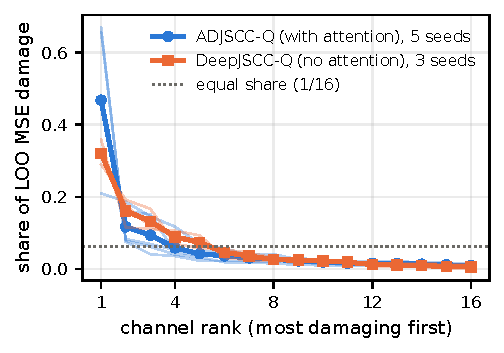
\includegraphics[width=\columnwidth]{figures/fig_profiles.pdf}
\caption{Sorted share of leave-one-out MSE damage per latent channel (thin: individual seeds; thick:
mean). Both architectures concentrate damage far above the equal share.}
\label{fig:profiles}
\end{figure}

\subsection{Where does tiered UEP gain come from?}
At 40\% loss uniform RS(96,64) fails in most images (\UniformForty~dB). The hand-designed 25/50/25 scheme
gains \HandTierGainForty~dB with the static LOO order, \HandTierAttentionGainForty~dB with attention and
\HandTierRandomGainForty~dB with a random order. A per-image LOO order (an unattainable upper bound) gains
\HandTierPerImageGainForty~dB. The unsorted two-tier control (two RS(48,32) blocks at the uniform rate)
isolates block length: \TwoTierUnsortedGainForty~dB at 40\% and \TwoTierUnsortedGainThirty~dB at 30\%. The
PET twin of the 25/50/25 scheme gains \PetTwinGainForty~dB, so sharing packets across tiers does not
rescue the hand-designed allocation. Below about 32\% loss the fixed scheme falls
behind uniform RS (\HandTierGainTwenty~dB at 20\%) because its bottom tier carries no parity.

\subsection{The optimal allocation is importance-ordered truncation}
Fig.~\ref{fig:main} and Table~\ref{tab:alloc} report the validation-optimized designs. Up to 20\% loss the
search returns uniform RS. From 30\% on it returns truncation (the top \TruncKeepThirty, \TruncKeepForty{}
and \TruncKeepFifty{} channels for 30, 40 and 50\% loss, each in one RS($96,4m$) block), or a PET or
three-level layout within a few tenths of a dB of it. Simulating the 25 surrogate-best genuinely multi-tier allocations improves on
truncation by at most \MultiTierMaxGain~dB on validation. PET designs are within \PetVsTruncMax~dB. On the
test split, truncation in LOO order gains \TruncOracleGainForty~dB at 40\% loss and
\TruncOracleGainFifty~dB at 50\%, about \TruncOverHandForty~dB more than the hand-designed scheme. It is
never worse than uniform RS at low loss, because there the selected design \emph{is} uniform RS.

The ranking now decides almost everything. With the same validation-chosen depth, truncation in random
order gains only \TruncRandomGainForty~dB at 40\% loss, in attention order \TruncAttentionGainForty~dB,
in energy order \TruncEnergyGainForty~dB, and with the 2,048-MAC head \TruncHeadGainForty~dB.
Proposition~\ref{prop:trunc} explains why: the coding gain of truncation is paid for by the damage of the
channels left out, which only an accurate ranking keeps small. The additive surrogate~\eqref{eq:surrogate}
predicts the simulated mean MSE of the test-evaluated layouts with Spearman correlation
\SurrogateSpearman{} and median relative error \SurrogateMedianRelErr\% (Fig.~\ref{fig:surrogate}), so the
allocation can be designed in closed form. The surrogate underestimates the MSE when many channels are
partially lost at once, because damage is mildly superadditive. It still ranks layouts well, and the final
choice is always made by exact simulation.

\begin{figure}[t]\centering
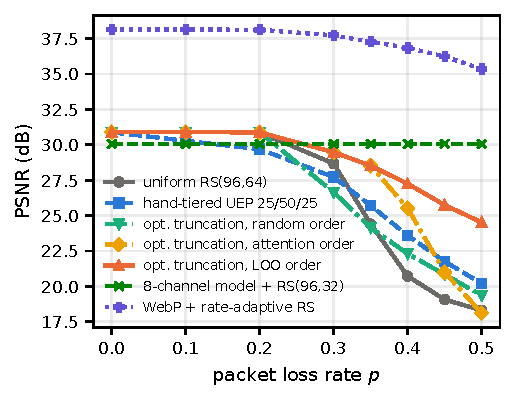
\includegraphics[width=\columnwidth]{figures/fig_main.pdf}
\caption{Test PSNR versus packet loss rate (1,536 transmitted bytes per image). Optimized allocations are
chosen per loss rate on validation. All curves except the 8-channel, ordered and WebP ones use the
primary model.}
\label{fig:main}
\end{figure}

\begin{table}[t]\centering\caption{Test PSNR (dB) and gain over uniform RS at 40\% loss}\label{tab:alloc}
\begin{tabular}{lrr}\toprule
Method & PSNR & gain\\\midrule
uniform RS(96,64) & \UniformForty & --\\
no RS (64 packets, 32 idle) & \NoRSForty & \NoRSGainForty\\
hand-tiered 25/50/25, LOO order & \HandTierForty & \HandTierGainForty\\
PET twin of 25/50/25 & \PetTwinForty & \PetTwinGainForty\\
Grad-FEC style (top 8 coded, 4 dropped) & \GradFecForty & \GradFecGainForty\\
opt.\ truncation, random order & \TruncRandomForty & \TruncRandomGainForty\\
opt.\ truncation, attention order & \TruncAttentionForty & \TruncAttentionGainForty\\
opt.\ truncation, energy order & \TruncEnergyForty & \TruncEnergyGainForty\\
opt.\ truncation, 2,048-MAC head & \TruncHeadForty & \TruncHeadGainForty\\
opt.\ truncation, LOO order & \TruncOracleForty & \TruncOracleGainForty\\
opt.\ grouped (multi-tier allowed) & \OptGroupedForty & \OptGroupedGainForty\\
opt.\ PET & \OptPetForty & \OptPetGainForty\\\bottomrule
\end{tabular}\end{table}

\begin{figure}[t]\centering
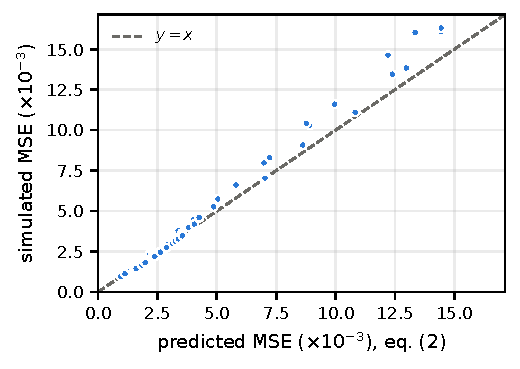
\includegraphics[width=\columnwidth]{figures/fig_surrogate.pdf}
\caption{Additive surrogate~\eqref{eq:surrogate} versus simulated mean MSE for every LOO-ordered layout and
loss rate evaluated on the test split.}
\label{fig:surrogate}
\end{figure}

\subsection{Unknown loss rate}
A design is only optimal at the loss rate it was made for. Fig.~\ref{fig:mismatch} shows the cost of
mismatch. A truncation designed for 40\% loss gives up \DesignFortyAtZeroLoss~dB on a clean channel and
gains \DesignFortyAtFifty~dB at 50\%. A single allocation optimized over $p\in[0.1,0.5]$ changes the PSNR by
\RobustGroupedGainForty~dB at 40\% and by \RobustGroupedGainTen~dB at 10\%. This is the only regime in which
the search selects a multi-level structure (the robust PET design: \RobustPetGainTen~dB at 10\%,
\RobustPetGainForty~dB at 40\%). With loss-rate feedback, the selector of Table~\ref{tab:alloc} (one byte
of signalling per loss-rate change) is the operating point we recommend.

\begin{figure}[t]\centering
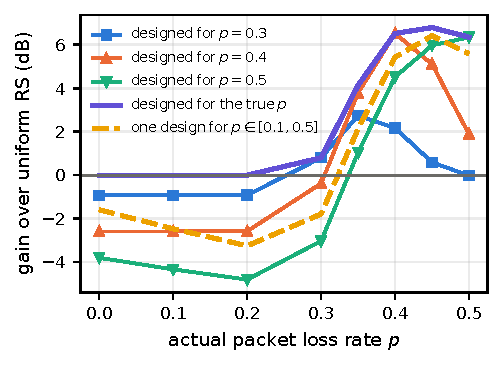
\includegraphics[width=\columnwidth]{figures/fig_mismatch.pdf}
\caption{Gain over uniform RS of allocations designed for one loss rate and used at another.}
\label{fig:mismatch}
\end{figure}

\subsection{Baselines that change the picture}
\emph{Smaller models.} Truncating a 16-channel model to $m$ channels competes with a model trained for
$m$ channels. With the same 96 packets, the 8-channel model (bandwidth ratio 1/12) behind RS(96,32) gives
\KnTwelveClean~dB at every loss rate up to 50\%: its code essentially never fails, and halving the latent
costs only about 0.8~dB of clean quality. The 6-channel model
behind RS(96,24) gives \KnSixteenForty~dB. Switching between such models dominates truncating an
unordered model at high loss. Truncation is the single-model approximation to this envelope, and its
quality is set by the ranking.

\emph{Ordered latents.} Nested (tail) dropout \cite{rippel2014nested} closes this gap with one network. During
training, half of the images keep only a uniformly random prefix of the 16 channels. The resulting LOO order
equals the channel index, and the clean cost is \OrderedCleanCost~dB. Truncation in index order then barely
depends on the loss rate: \OrderedTruncForty~dB at 40\% and \OrderedTruncFifty~dB at 50\% loss. On the same
model, uniform RS gives \OrderedUniformForty~dB and truncation in random order \OrderedRandomForty~dB at
40\%. The ordered model is above the 8-channel model at every loss rate. The DeepJSCC-Q counterpart
behaves the same (\OrderedDeepTruncForty~dB at 40\%, \OrderedDeepClean~dB clean). In the ordered ADJSCC-Q
model the last five channels carry almost nothing (each LOO drop at most 0.02~dB). Nested dropout thus
trades unused capacity for an embedded order, which is exactly what classical ULP assumes.

\emph{No RS at all.} A 24-channel model can spend all 1,536 bytes on latent symbols and be fine-tuned
over packet erasures, so that it degrades gracefully without any code. None of three 24-channel ADJSCC-Q
runs converged under our recipe (best clean validation PSNR \NoRsBestValClean~dB, below the 16-channel
model). The DeepJSCC-Q recipe did converge, so we compare within it.
\begin{itemize}
\item \emph{No RS, 24 channels, erasure fine-tuned:} \NoRsDeepForty~dB at 40\% loss (\NoRsDeepClean~dB clean).
\item \emph{RS with LOO truncation, 16 channels:} \RsDeepTruncForty~dB at 40\% (\RsDeepClean~dB clean).
\item \emph{The same, after the same fine-tuning:} \RsDeepRobustTruncForty~dB at 40\%.
\end{itemize}
Without RS the quality falls from the first lost packet (\NoRsDeepThirty~dB at 30\%, against
\RsDeepTruncThirty~dB). Packet-level RS with truncation is therefore the better use of the budget up to
45\% loss. At 50\%, the fine-tuned no-RS model (\NoRsDeepFifty~dB) passes truncation of the plain model
(\RsDeepTruncFifty~dB) but not of the fine-tuned one (\RsDeepRobustTruncFifty~dB).

\emph{Conventional codecs.} Earlier comparisons in this line gave JPEG, JPEG2000 and WebP a fixed
RS(96,64) code, which collapses beyond 33\% loss (WebP: \WebpFixedForty~dB at 40\%). Allowed the same
choice we give the JSCC transmitter, i.e.\ fewer source bytes and a stronger code chosen on validation, WebP
keeps \WebpAdaptiveForty~dB at 40\% and \WebpAdaptiveFifty~dB at 50\% loss, above every JSCC system
here (clean: \WebpAdaptiveZero~dB versus \CleanPsnr~dB). At this rate, byte-quantized JSCC without entropy
coding is far from codec efficiency. Our conclusions are about how to protect a learned latent once it
is the transmitted representation, not about JSCC versus separation.

\subsection{Across model seeds and architectures}
Table~\ref{tab:seeds} repeats the main comparison for every converged model, each with its own LOO
ranking and validation-chosen truncation depth. LOO-ordered truncation gains \TruncGainMinAdj{} to
\TruncGainMaxAdj~dB over uniform RS at 40\% loss for ADJSCC-Q and \TruncGainMinDeep{} to
\TruncGainMaxDeep~dB for DeepJSCC-Q, and beats the hand-tiered scheme on every model
(\TruncOverHandMinAll{} to \TruncOverHandMaxAll~dB). The primary model is the most favourable ADJSCC-Q
seed. Energy order is within 0.9~dB of LOO order on every model, while attention order is unreliable:
it ranges from below the random order (ADJSCC-Q seed 21) to 1.5~dB under LOO order.
\begin{table}[t]\centering\caption{Test PSNR (dB) at 40\% loss across models}\label{tab:seeds}
\resizebox{\columnwidth}{!}{% generated by experiments/paper_figures.py -- do not edit
\begin{tabular}{lrrrrrrr}
\toprule
model & clean & uniform & hand-tiered & \multicolumn{4}{c}{opt.\ truncation, order:} \\
 & & & LOO & LOO & energy & attention & random \\
\midrule
ADJSCC-Q s100 & 31.34 & 20.77 & 23.60 & 25.77 & 25.75 & 23.15 & 22.28 \\
ADJSCC-Q s13 & 31.76 & 20.64 & 23.54 & 26.18 & 26.36 & 22.41 & 22.13 \\
ADJSCC-Q s21 & 31.09 & 20.79 & 23.90 & 26.14 & 25.27 & 20.78 & 22.24 \\
ADJSCC-Q s42 & 30.88 & 20.73 & 23.59 & 27.25 & 26.72 & 25.72 & 22.42 \\
ADJSCC-Q s7 & 31.45 & 21.02 & 23.37 & 25.04 & 25.74 & 23.25 & 22.70 \\
DeepJSCC-Q s100 & 31.79 & 18.56 & 22.19 & 28.00 & 27.89 & -- & 20.54 \\
DeepJSCC-Q s21 & 32.73 & 19.52 & 22.70 & 25.63 & 26.03 & -- & 21.51 \\
DeepJSCC-Q s7 & 32.17 & 17.81 & 21.86 & 26.03 & 26.08 & -- & 19.64 \\
\bottomrule
\end{tabular}
}
\end{table}

\section{Discussion and Limitations}
The study uses $32{\times}32$ images, one bandwidth ratio for the primary analysis, i.i.d.\ losses for the
allocation results, and a known loss rate for the selector. Under Gilbert--Elliott bursts with 45\% average
loss, LOO truncation still beats uniform RS, by \BurstTruncGainOne~dB with i.i.d.\ losses and by
\BurstTruncGainSixteen~dB at a mean burst length of 16 packets. The interleaved hand-tiered scheme gains
\BurstHandGainOne~dB and \BurstHandGainSixteen~dB respectively. Choosing the truncation depth for the burst
statistics adds at most \BurstDepthGainMax~dB. The SSIM implementation of the code base uses zero-padded
windows, so we report PSNR only. Two of five DeepJSCC-Q seeds and one of six ADJSCC-Q seeds did not
converge under the common recipe; they are excluded by a rule fixed before evaluation.


% =====================================================================================================
\section{Conclusion}
Protecting a quantized Deep JSCC latent with packet-level RS is less a question of how many protection
levels to use than of which latent bytes to send at all. Erasure sensitivity is concentrated, reproducible
across seeds and present without attention modules. The backbone's SNR-conditioned attention gates do not
predict it, while latent energy and a 2,048-MAC head do. Because RS is MDS, the outcome of any systematic
layout is exact and its expected distortion has an accurate closed-form surrogate. With it, the optimal
allocation at a known loss rate turns out to be importance-ordered truncation with one strong code, which
outperforms hand-designed multi-tier UEP by several dB and depends almost entirely on the quality of the
ranking. Multi-level codes help only when one allocation must serve many loss rates. When the order is
imposed by nested dropout, truncation keeps nearly the clean quality up to 50\% loss with a single network,
above a model trained for the smaller bandwidth. With the same erasure fine-tuning, RS with truncation also beats
spending the whole budget on latent bytes without RS. Conventional codecs with rate-adaptive RS remain stronger on
CIFAR-10. Closing that gap (entropy-coded latents, higher resolutions) is the natural next step.


\bibliographystyle{IEEEtran}
\bibliography{references}
\end{document}
